%!TEX root = ../report.tex

\chapter{ State of the Art }

Given the range of the different methods for implementing a spatio-temporal
world model, the methods have been divided into groups.  Most spatio-temporal
world models are implemented on top of preexisting world modeling techniques
and thus the majority of implementations are tied to a specific spatial
representation. There are, however, exceptions to this with some models being
built from the ground up effectively intertwining the spatial and temporal
components. On the opposite end of this spectrum, there exists currently at
least one method that can be used in combination with a multitude of different
world models.


\section{ Map Dependent Models }

\subsection{ Occupancy Grids }

Occupancy grids were introduced in 1985 by Moravec and Elfes. \cite{Elfes1985}
In simple two dimensional terms, they can be thought of as a grid placed
over an environment. Each cell then represents the probability or belief that
that that cell is either occupied or free. Free in the simplest case meaning
that a robot would be able to traverse through the cell. This concept can of
course be extended into the third dimension for a more complex world model. \\

\subsubsection{ Temporal Occupancy Grids }
One of the earliest and most straight forward attempts to introduce a temporal
component to a world model were by extending existing world models, occupancy
grids in particular. This can be seen in Temporal Occupancy Grids: a Method for
Classifying the Spatio-Temporal Properties of the Environment.
\cite{Arbuckle2002} In this paper Arbuckle et al introduce the concept of
temporal occupancy grids (TOGs). The authors noted that the key to these TOGs
were that they "can differentiate between different patterns of occupancy, even
when the absolute probability of occupancy is the same." That is to say, one
could imagine a parking lot where it would be possible with TOGs to distinguish
between cells that are parking spaces, cells that are pathways, and cells that
are not for driving at all, such as a median. These TOGs additionally made it
possible to detect where a door or elevator may be. \\

Temporal Occupancy Grids were accomplished by generated multiple occupancy
grids in the same fashion as was traditionally done but each occupancy grid
would represent, and be generated using samples from, multiple different time
scales. With multiple occupancy grids spanning multiple time scales, the
probability of a cell being occupied could be computed by a simple summation.

\subsubsection{ Hidden Markov Models }

Hidden Markov Models (HHMs), are a type of Markov Chain that can be considered
"a doubly embedded stochastic process with an underlying stochastic process
that is not observable (it is hidden), but can only be observed through
another set of stochastic processes that produce the sequence of observations."
\cite{Rabiner1989}. In more general terms, an HMM can be though of as having N
number of states S, that are hidden, or otherwise not directly observable.
Each state can have M observations made about properties of these states which
may reflect indirectly, to varying degrees of certainty, the actual state.
Furthermore, each one of these states has a given probability distribution of
transitioning from one state to another. It is from this information that a
Markov Model or Markov Chain can be constructed. \\

TODO: Add image? \\

In the specific case of occupancy grids, each cell can be thought of having two
states, free, and occupied. It is not feasible to be able to directly observe
every given cell at all times, and specifically at the time of path planning
and thus there states can be thought of as hidden. However, through past
observation and data collection, there is data know about a cell throughout
time. Thus this temporal data can be thought of as the observational data and
be used to make predictions about state transitions. \\

Early combinations of HMMs with occupancy grids differed from previous dynamic
world modeling approaches as this approach "does not depend on dynamic object
detection and high-level object models; it considers only the occupancy of the
space at a lower level of abstraction"\cite{Meyer-Delius2012}. By relying on
and collecting lower, more easily observable data, larger amounts of data could
be collected and processed over greater periods of time. Since each cell was
dependent only on previous observations of that cell throughout time, the
increase in data quantity and the discrete nature of the predictions lent
themselves would improve state predictions. \\

Meyer-Delius \cite{Meyer-Delius2012} also introduced the concept of online
learning to this approach. Traditionally, offline learning had been used where
a robots navigational system would hold copy of a world model produced a some
time before operation. It has possible that from the time the map was generated
to the time at which the robot was operating that objects in the robots
environment may have changed. With the introduction of online learning, the
robot would be able to observe these changes and factor them in to its
navigational system. This was the first addition to attempt to avoid the static
nature of the transition states of the HMM. \\

Further improvement to occupancy grids with HMMs came with the concept of
modeling trajectories of objects in the environment\cite{Wang2015}. This is an
important improvement because the dynamic motion of objects in an environment,
such as humans walking a hallway, could now be better modeled. This process
was dubbed Input-Output HMM (IOHMM) due nature of how cells of the grid would
communicate with one another. Each cell would not only look through it's own
historical data but also be able to communicate with its neighbors. In effect,
this could allow a cell in hallway to be able to predict occupancy based off of
a nearby cell that is currently occupied.

\subsection{ Spatio-Temporal Hilbert Maps }

In contrast to the discrete nature of occupancy grids, Hilbert maps provide a
continuous representation of an environment which allows for arbitrary world
model resolution. They rely on "fast kernel approximations that project the
data in a Hilbert space where a logistic regression classifier is learnt"
A stochastic gradient optimization can then applied. This approach is similar to
that of a Gaussian processes occupancy map but with a much lower computational
cost computational cost computational cost computational cost. Having been
introduced as recently as 2016, Hilbert maps, and the addition of a temporal
component, are still a fairly new field of research but already some of the
authors from the original paper have already begun to introduce a temporal
component to this new form of world model. \cite{Ramos2016, Senanayake2016} \\

In static Hilbert maps, the kernel can be thought of as the location of an
obstacle or object. When introducing the temporal dimension, the centroid of a
moving object is extracted from raw data over time. This data can the be used
and trained on to create a model that can predict the direction and speed of an
object at a given location at a given time. It is particularly well suited to
short-term predictions such as car traffic on a road or at an intersection.
\cite{Senanayake2016} \cite{Senanayake2017}

\begin{figure}
  \centering
  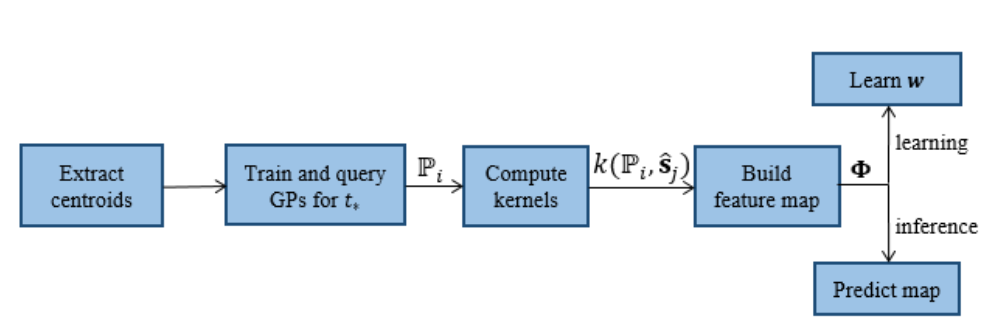
\includegraphics[width=\linewidth]{images/STHM_diag.png}
  \caption{Spatio-temporal Hilbert map training process (GP - Gaussian Process)}
  \cite{Senanayake2016}
  \label{figure:example}
\end{figure}

\section{ Map Independent Models }
\subsection{ FreMen }
\subsubsection{ Poisson-Spectral Models }


\section{ Existing Methods for Evaluation or Comparison }

\subsection { Example 1 }
\subsection { Example 2 }


CITATION \cite{art1}.
\section{Limitations of previous work}
